\documentclass[a4paper,12pt,headsepline]{report}

%----------------- PDF CONFIG ----------------- %
\pdfinfo{    
     /Title (Permissioned Blockchains für B2B - Prototypische Implementierung eines dezentralisierten Wartungsmarktes) 
     /Subject   (Permissioned Blockchains)    
     /Author  (Eric Nagel) 
     /Keywords   (Blockchain, B2B)      
}

\title{Permissioned Blockchains für B2B - Prototypische Implementierung eines dezentralisierten Wartungsmarktes}
\author{Eric Nagel}
\date{09.03.2018}



%----------------- PAKETE INKLUDIEREN ----------------- %

\usepackage{geometry} % Packet für Seitenrandabständex und Einstellung für Seitenränder
\usepackage[ngerman]{babel} % deutsche Silbentrennung

\usepackage{booktabs} %entzerrt die Tabellenzeilen und bietet verschieden dicke Unterteilungslinien
\usepackage{longtable} % Tabellen können sich nicht über mehrere Seiten 
\usepackage{graphicx} % kann LaTeX Grafiken einbinden

\usepackage[utf8]{inputenc}
\usepackage[T1]{fontenc} % Zeichenencoding
\usepackage{lmodern} % typographische Qualität 
\frenchspacing % Schaltet den zusätzlichen Zwischenraum ab
\usepackage{fix-cm}
\usepackage{hyperref} % verwandelt alle Kapitelüberschriften, Verweise aufs Literaturverzeichnis und andere Querverweise in PDF-Hyperlinks
\usepackage{color}
\usepackage{url}
\usepackage{enumitem}
\setitemize{itemsep=0pt}

\usepackage[nottoc]{tocbibind}

% für Listings
\usepackage{listings}
\lstset{numbers=left, numberstyle=\tiny, numbersep=5pt, stepnumber=4, keywordstyle=\color{black}\bfseries\itshape, stringstyle=\ttfamily,showstringspaces=false,basicstyle=\footnotesize,captionpos=b}
\lstset{language=java}

%----------------- FARBEN DEFINIEREN ----------------- %
\definecolor{gray}{gray}{0.95} % Listingsbackground

%----------------- LAYOUT SETZEN ----------------- %
\geometry{left=2cm, right=2cm, top=2.5cm, bottom=2cm}
\linespread {1.25}\selectfont %1.25 da er von Haus aus 1.2 ist und 1,25 * 1,2 = 1,5 isch

%%----------------- INHALT -----------------%
\begin{document}

\pagenumbering{roman} % Seitennummer

 %----------------- KONFIGURATION ----------------- %
\pagestyle{empty} % enthalten keinerlei Kopf oder Fuß 

%----------------- HDA FBI Logo ----------------- %
\begin{figure}[t]
	\centering
	
\includegraphics[width=0.6\textwidth]{images/logo_fbi}
\end{figure}

%----------------- INHALT ----------------- %

\begin{center}
\Large Hochschule Darmstadt \\
\normalsize \textsc{- Fachbereich Informatik -} \\

% Whitespace
\vspace{80 pt}

\Huge Permissioned Blockchains für B2B \\ 
\Large Prototypische Implementierung eines dezentralisierten Wartungsmarktes \\
\normalsize
\vspace{20 pt}

Abschlussarbeit zur Erlangung des akademischen Grades \\ 
Bachelor of Science (B.Sc.) 

\vspace{75 pt}


vorgelegt von \\
\vspace{5 pt}
Eric Nagel \\
Matrikelnummer 740693
\vspace{80 pt}

\begin{tabular}[h]{p{4cm}l l}
	Referent: & Prof. Dr. Andreas Müller \\
	Korreferent: & Björn Bär
\end{tabular}


\end{center}


 %----------------- KONFIGURATION ----------------- %
\pagestyle{empty} % enthalten keinerlei Kopf oder Fuß

%TODO: Abstract eventuell auf 3/4 Seite verlängern
\chapter*{Zusammenfassung} % (fold)
\addcontentsline{toc}{chapter}{Zusammenfassung}
\label{cha:abtract}

Traditionelle B2B-Anwendungen, mit multiplen Unternehmen als Teilnehmer, bringen Probleme bezüglich der Datenhaltung mit sich. Eine Option ist, dass jedes Unternehmen Daten bei sich selber speichert. Dies führt jedoch zu zusätzlichen Aufwand, da Schnittstellen eingerichtet werden müssen, um Geschäftspartnern Zugriff auf relevante Daten zu gewähren. Eine weitere Option ist die Speicherung bei einer zentralen, verwaltenden Instanz. Jeder Geschäftspartner müsste dieser jedoch vertrauen, was die Anwendung unattraktiver macht. Eine Lösung für diese Probleme könnte die Blockchain-Technologie darstellen. Mit ihr ist eine verteilte Datenspeicherung unter nicht vertrauenswürdigen Teilnehmern möglich. Dabei stellt die Blockchain sicher, dass die Daten bei allen Geschäftspartnern synchron sind, und nicht manipuliert oder gelöscht werden können. Die Technologie bringt jedoch auch Schwierigkeiten mit sich, welche für B2B-Anwendungen unerwünscht sind. In Public Blockchains wie Bitcoin und Ethereum äußert sich dies anhand der Skalierbarkeit, Performance und Sicherheit. Permissioned Blockchains, wie Hyperledger Fabric, können diese Probleme zu Teilen lösen. Nichtsdestotrotz sind darauf basierende Anwendungen auf eine bestimmte Performance oder Nutzerzahl limitiert. Auf Grundlage dieser Erkenntnisse wurde ein Prototyp eines automatisierten dezentralen Wartungsmarktes als Proof-of-Concept entwickelt. In diesen können IoT-Geräte Wartungsbedarf erkennen und Wartungsanbieter darauf reagieren.

 
\tableofcontents % Inhaltverzeichnis

\listoffigures % Abbildungen

\listoftables % Tabellen

\renewcommand{\lstlistlistingname}{Listingverzeichnis}
\lstlistoflistings

\pagestyle{plain} % zurueck setzen von roemische seitenanzahl

\pagenumbering{arabic}
\chapter{Einführung und Motivation}
\label{cha:einfuehrung}

\begin{itemize}
    \item Entwicklung eines dezentralen Wartungsmarktes
    \item Wozu ein dezentraler Wartungsmarkt ? Klassische B2B-Anwendungen und deren Probleme beschreiben (Viele Kooperationsverhandlungen, evtl. herausbilden einer neuen kontrollierenden Instanz, Sensible Daten bei anderen Unternehmen) 
  
     \begin{itemize}
      \item Daten bei jeden Unternehmen, aufwändiger Zugriff, unterschiedliche Datenformate, etc.
      \item Alle Daten zentral bei einer Instanz (Evtl. auch sensible Daten)
      \item Partner schrecken wegen Nichtvertrauen zurück
      \item Zugriff aufwändig über APIs
    \end{itemize}
    \item Lösung: Blockchain, kurz Kernelemente nennen
    \item Probleme bekannter Blockchain-Technologien für B2B-Zwecke nennen
    \item Technologien und Arten(Permissioned/Public) erwähnen, welche diese Probleme lösen sollen
    \item Theoretische und praktische Analyse durch Implementation eines dezentralisierten Wartungsmarktes (Genauer beschrieben), welcher die Probleme von klassischen B2B-Anwendungen löst.
    \item Ziel der Arbeit: Implementierung des dezentrales Wartungsmarktes beschreiben, und in Zuge dessen den Nutzen der Blockchain-Technologie im B2B-Bereich evaluieren sowie die Anwendung darauf untersuchen
    \item Vorgehen:
    \begin{itemize}
      \item Blockchain Grundlagen erklären
      \item Dezentralen Wartungsmarkt und die Anforderungen an diesen erklären
      \item Nachteile der Blockchain und Auswirkung auf B2B-Bereich nennen 
      \item Theoretische Analyse, ob die Probleme gelöst werden können
      \item Implementierung des dezentralen Wartungsmarktes beschreiben
      \item Fazit/Ausblick zur Lösung der Probleme und des entwickelten Systems geben
    \end{itemize}
  \end{itemize}

  \cite{WustyouneedBlockchain2017}

\pagenumbering{arabic}
\chapter{Grundlagen}
\label{cha:grundlagen}

\section{Blockchain}

\subsection{Funktion}
\subsection{Probleme für den B2B-Bereich}

\section{Klassische B2B-Anwendungen}
	
\include{structure/wartungsmarkt-konzept}
\pagenumbering{arabic}
\chapter{Related Work}
\label{cha:related-work}



\pagenumbering{arabic}
\chapter{Evaluierung Permissioned Blockchains für B2B}
\label{cha:b2b-eval}



\pagenumbering{arabic}
\chapter{Dezentraler Wartungsmarkt - Implementierung}
\label{cha:wartungsmarkt-impl}


\pagenumbering{arabic}
\chapter{Fazit}
\label{cha:fazit}





%----------------- KAPITEL : BEISPIELE  ----------------- %	
% \chapter{Beispiele}
% \label{cha:beispiele}
% 	Dieses Kapitel soll viele alltaegliche Beispiele\footnote{Fussnote} abdecken um einen {\LaTeX} Dokument zu setzen \cite{WustyouneedBlockchain2017}

% 		\section{Schriftarten}
% 		\label{sec:schriftarten} 
% 			\begin{itemize}
% 				\item Kursiv: \emph{Das ist ein Beispiel}
% 				\item Unterstreichen: \underline{Das ist ein Beispiel}
% 				\item Fettschrift: \textbf{Das ist ein Beispiel}
% 				\begin{itemize} 
% 					\item Kombination aus dreien: \underline{\textbf{\emph{Das ist ein Beispiel}}}						\end{itemize} 
% 				\item Serifen: \textsf{Das ist ein Beispiel}
% 				\item Schreibmaschinen Schrift: \texttt{Das ist ein Beispiel}
% 				\item Kleine Grossbuchstassen: \textsc{Das ist ein Beispiel}
% 				\item Ausfuehrungszeichen: ``Das ist ein Beispiel''
% 				\item asld
% 			\end{itemize}
			
		
			
				

% 	\section{Abbildungen}
% 		Wie folgt bindet man Abbildungen ein:
% 		% Beispiel für Bildintegration
% 		\begin{figure}[htb]
% 		 \centering
% 		 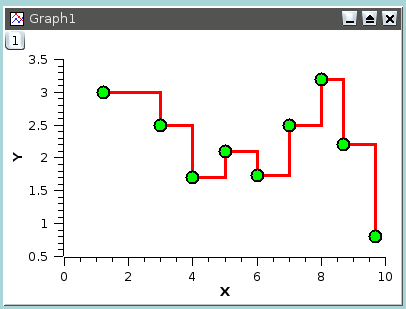
\includegraphics[width=0.4\textwidth,angle=0]{images/beispiel}
%  		\caption{Beispiel Bild; Quelle ist png}
% 		\label{fig:beispiel}
% 		\end{figure}
	
% 	\section{Tabellen}
% 			Lorem ipsum dolor sit amet, consetetur sadipscing elitr, sed diam nonumy eirmod tempor invidunt ut labore et dolore magna aliquyam erat, sed diam voluptua. At vero eos et accusam et justo duo dolores et ea rebum. Stet clita kasd gubergren.

% 		\begin{center}
% 			\begin{tabular}{lcrc} \toprule
% 			Stadium & Substratfreie Kontrolle  & \multicolumn{2}{c}{Probenansatz} \\\cmidrule(rl){3-4}
% 			 & Farbe & Farbe & Bewertung \\\midrule
% 			Alpha1 & farblos & braun & +++ \\
% 			Beta2 & farblos & farblos & - \\\bottomrule 
% 			 \end{tabular}
% 		 \end{center}
		 
% 		2. Beispiel \\
% 		\begin{table}[h]
% 		\centering	 
% 		 	\begin{tabular}{|l|l|c|}
% 			\hline
% 			\textsc{Rang} & \textsc{Name} & \textsc{Rating}\\
% 			\hline
% 			\hline
% 			1 & Garry Kasparov & 2817\\
% 			2 & Viswanathan Anand & 2774\\
% 			3 & Wladimir Kramnik & 2764\\
% 			\hline
% 			\end{tabular}
% 		\caption{Beispiel Beschriftung einer Tabelle}
% 		\label{tab:beispiel}
% 		\end{table}
		
		


% 	\section{Verweise}
% 		Hier werden Verweise auf verschiedene Elemente erstellt.
% 		\subsection{Pageref und Ref} 
% 			Diese Textstelle ist sehr interessant.\label{interessant} \\				
% 			Hier wird auf die Textstelle~\ref{interessant} verwiesen, \\
% 			die sich auf der Seite~\pageref{interessant} befindet.\\[20pt] 
% 			Verweis auf Listing \ref{lst:javaBsp} auf Seite \pageref{lst:javaBsp} \\
% 			Verweis auf Abbildung \ref{fig:beispiel} auf Seite \pageref{fig:beispiel} \\
% 			Verweis auf Tabelle \ref{tab:beispiel} auf Seite \pageref{tab:beispiel}
			
% 	\section{Listing}
% 		\lstset{language=java}
% 		\begin{lstlisting}[frame=hl, caption={Das Listing zeigt Java Quellcode} ,backgroundcolor=\color{gray}, label={lst:javaBsp}]
% /* Java Hallo World Beispiel */

% public class HelloWorld {
%     public static void main(String[] args) {
%         System.out.println("Hello, World");
%     }
% }
% 		\end{lstlisting} 
		
	
\bibliographystyle{plain}
\bibliography{literature}
\pagenumbering{Roman}	
	

	
\end{document}